\begin{solution}
    \begin{enumerate}[label = \Alph*)]
        \item After calculating the excess returns for the \(N = 38\) industry portfolios, the remaining dataset contains \(T = 15265\) daily returns. Using \(k = 1, \dots, 10\) principal components, I calculate the total explained variance ratio for each of the models. This is shown in Figure~\ref{fig:pca_criteria}. As we see, the variance ratio increases monotonically with the number of factors, something that is explained by the nature of the PCA.
        
        Assuming that the idiosyncratic returns (a.k.a. residuals) are normally distributed, independent over time and with a fixed covariance matrix between industries, the log-likelihood function is given by
        \[
            \log\Lc\bs{\bp{\varepsilon_{j,t}}_{j = 1,\dots,N; t = 1, \dots, T}} = -\frac{NT}{2}\log{2\pi} - \frac{T}{2}\log{\det\of\Sigma} - \frac{1}{2}\sum_{t = 1}^{T}\varepsilon_t^\prime\Sigma^{-1}\varepsilon_t,
        \]
        Estimating \(\Sigma\) from the time series of residuals I can calculate both the Akaike and the Schwarz Information Criteria (AIC and BIC, respectively) as:
        \begin{align*}
            AIC(k) & = 2k - 2 \log\Lc \\
            BIC(k) & = k\log{NT} - 2 \log\Lc
        \end{align*}
        These are ploted along the explained variance in Figure~\ref{fig:pca_criteria}. As it is usual with these measures, they tend to indicate a way more parsimonious model, with maximum criteria being achieved at only 1 factor for all measures.
        \begin{figure}[!htbp]
            \begin{small}
                \begin{center}
                    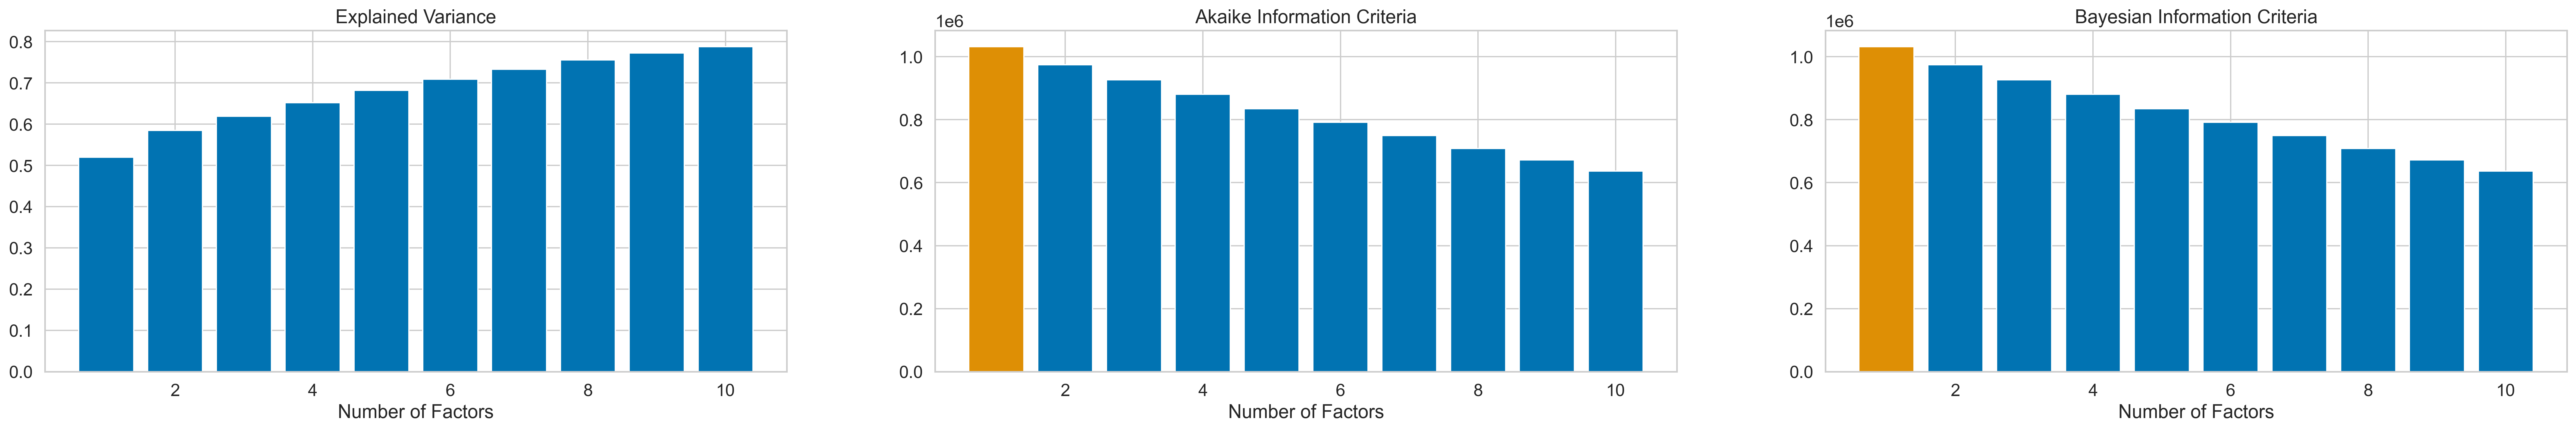
\includegraphics[width=\textwidth]{pca_criteria.png}
                \end{center}
                \caption{Explained Variance, AIC and BIC as a function of the number of factors}
                \label{fig:pca_criteria}
            \end{small}
        \end{figure}

    \item Using the model with 10 factors, I calculate the correlation matrix between the principal components and the Fama-French factors. This is shown in Figure~\ref{fig:pca_ff_corr}. As the figure shows, the first component is highly correlated with the market factor, meaning that the market portfolio is responsible for most of the variation in the industry portfolios. This gets clearer when we look at Figure~\ref{fig:pca_vs_market} which shows the time series of the Market and PC1. The two series very much like each other, indicating that indeed Market is the most important factor. On the other components, PC3 looks to correlate with HML, SMB and CMA. PC4 has high correlation with the Small minus Big (SMB) factor. Finally, the 7th component strongly correlates with the value factor (HML). The other components do not display significant correlation with any of the FF factors.
    
    \begin{figure}[!htbp]
        \begin{small}
            \begin{center}
                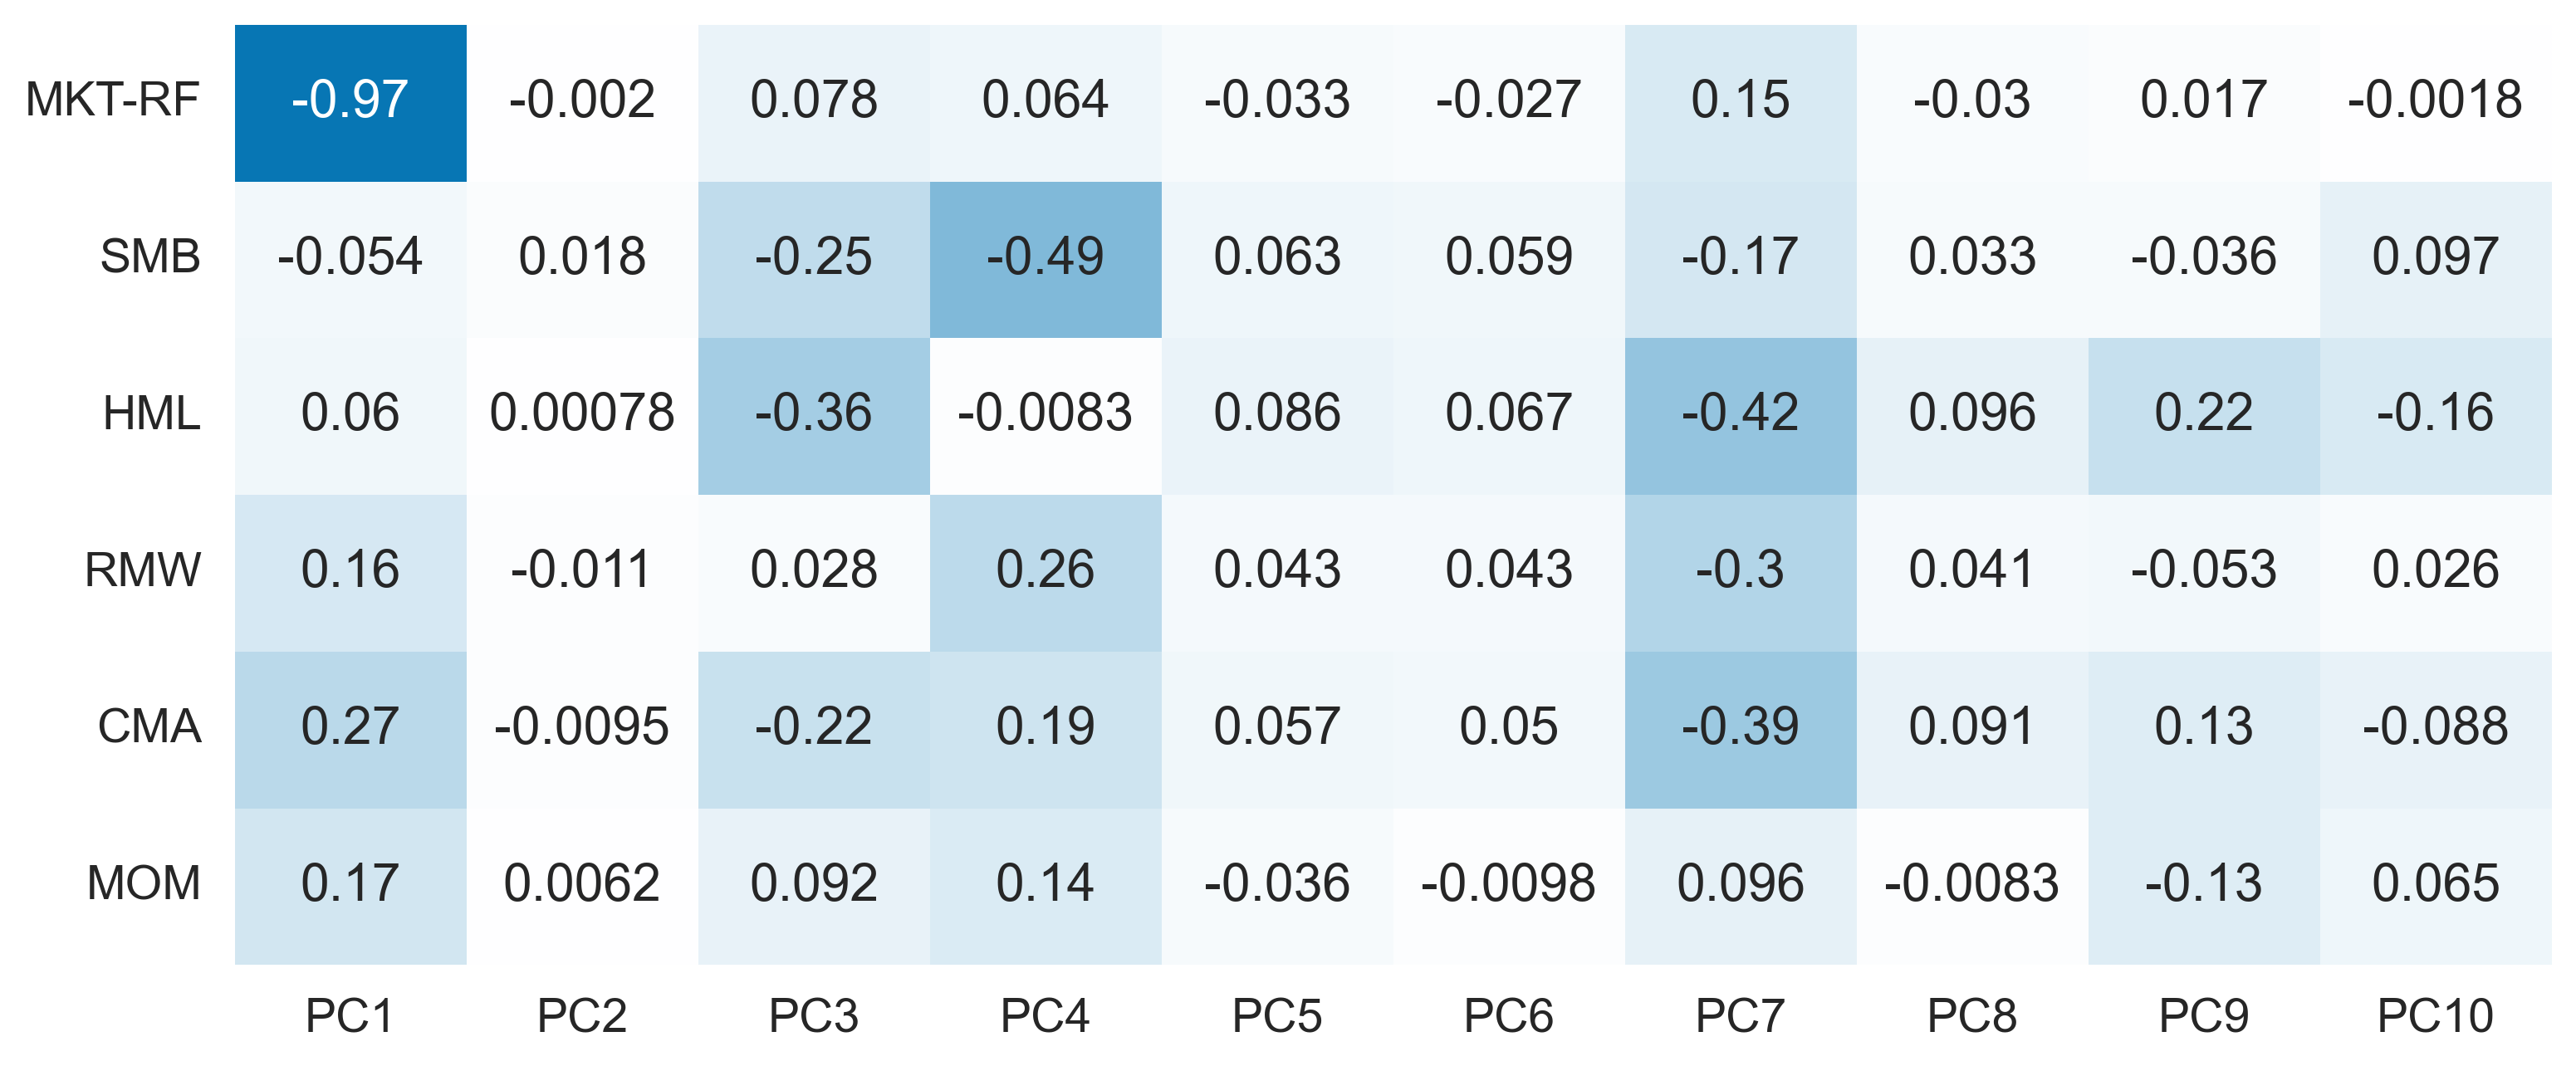
\includegraphics[width=0.8\textwidth]{factor_corr.png}
            \end{center}
            \caption{Correlation between Principal Components and FF}
            \label{fig:pca_ff_corr}
        \end{small}
    \end{figure}
    
    \begin{figure}[!htbp]
        \begin{small}
            \begin{center}
                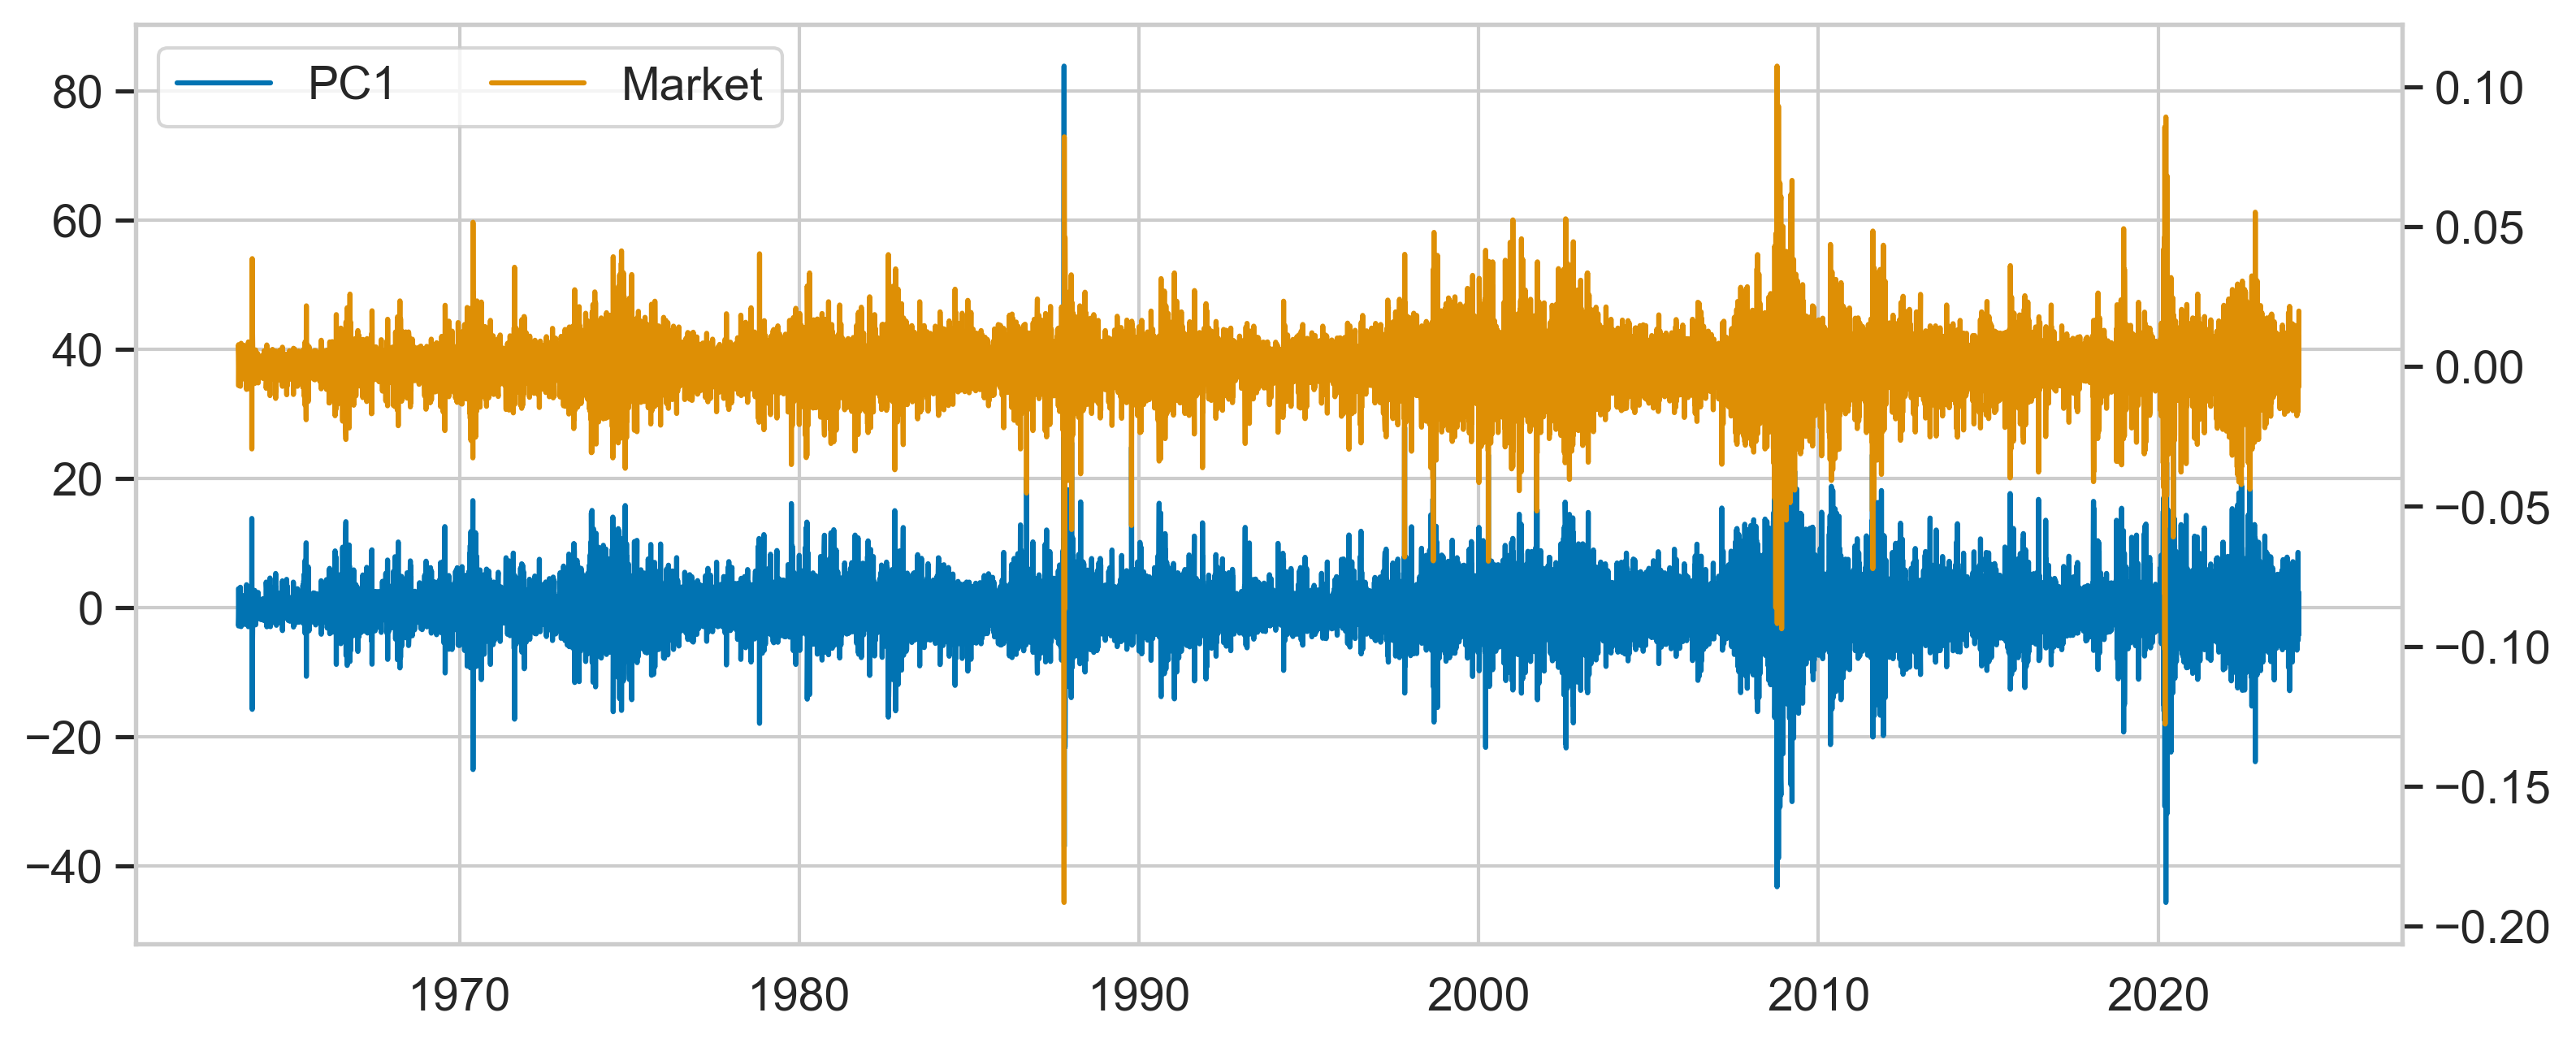
\includegraphics[width=0.8\textwidth]{pca_vs_market.png}
            \end{center}
            \caption{PC1 and Market Portfolio}
            \label{fig:pca_vs_market}
        \end{small}
    \end{figure}
    
    \item Using \(c = 1, \dots 5\), I calculate the canonical correlation between the PC and the FF factors. The CCA score, or canonical correlation, is shown in Figure~\ref{fig:cca_score}. As we see, the highest canonical correlation is achived with 3 components.  
    \begin{figure}[!htbp]
        \begin{small}
            \begin{center}
                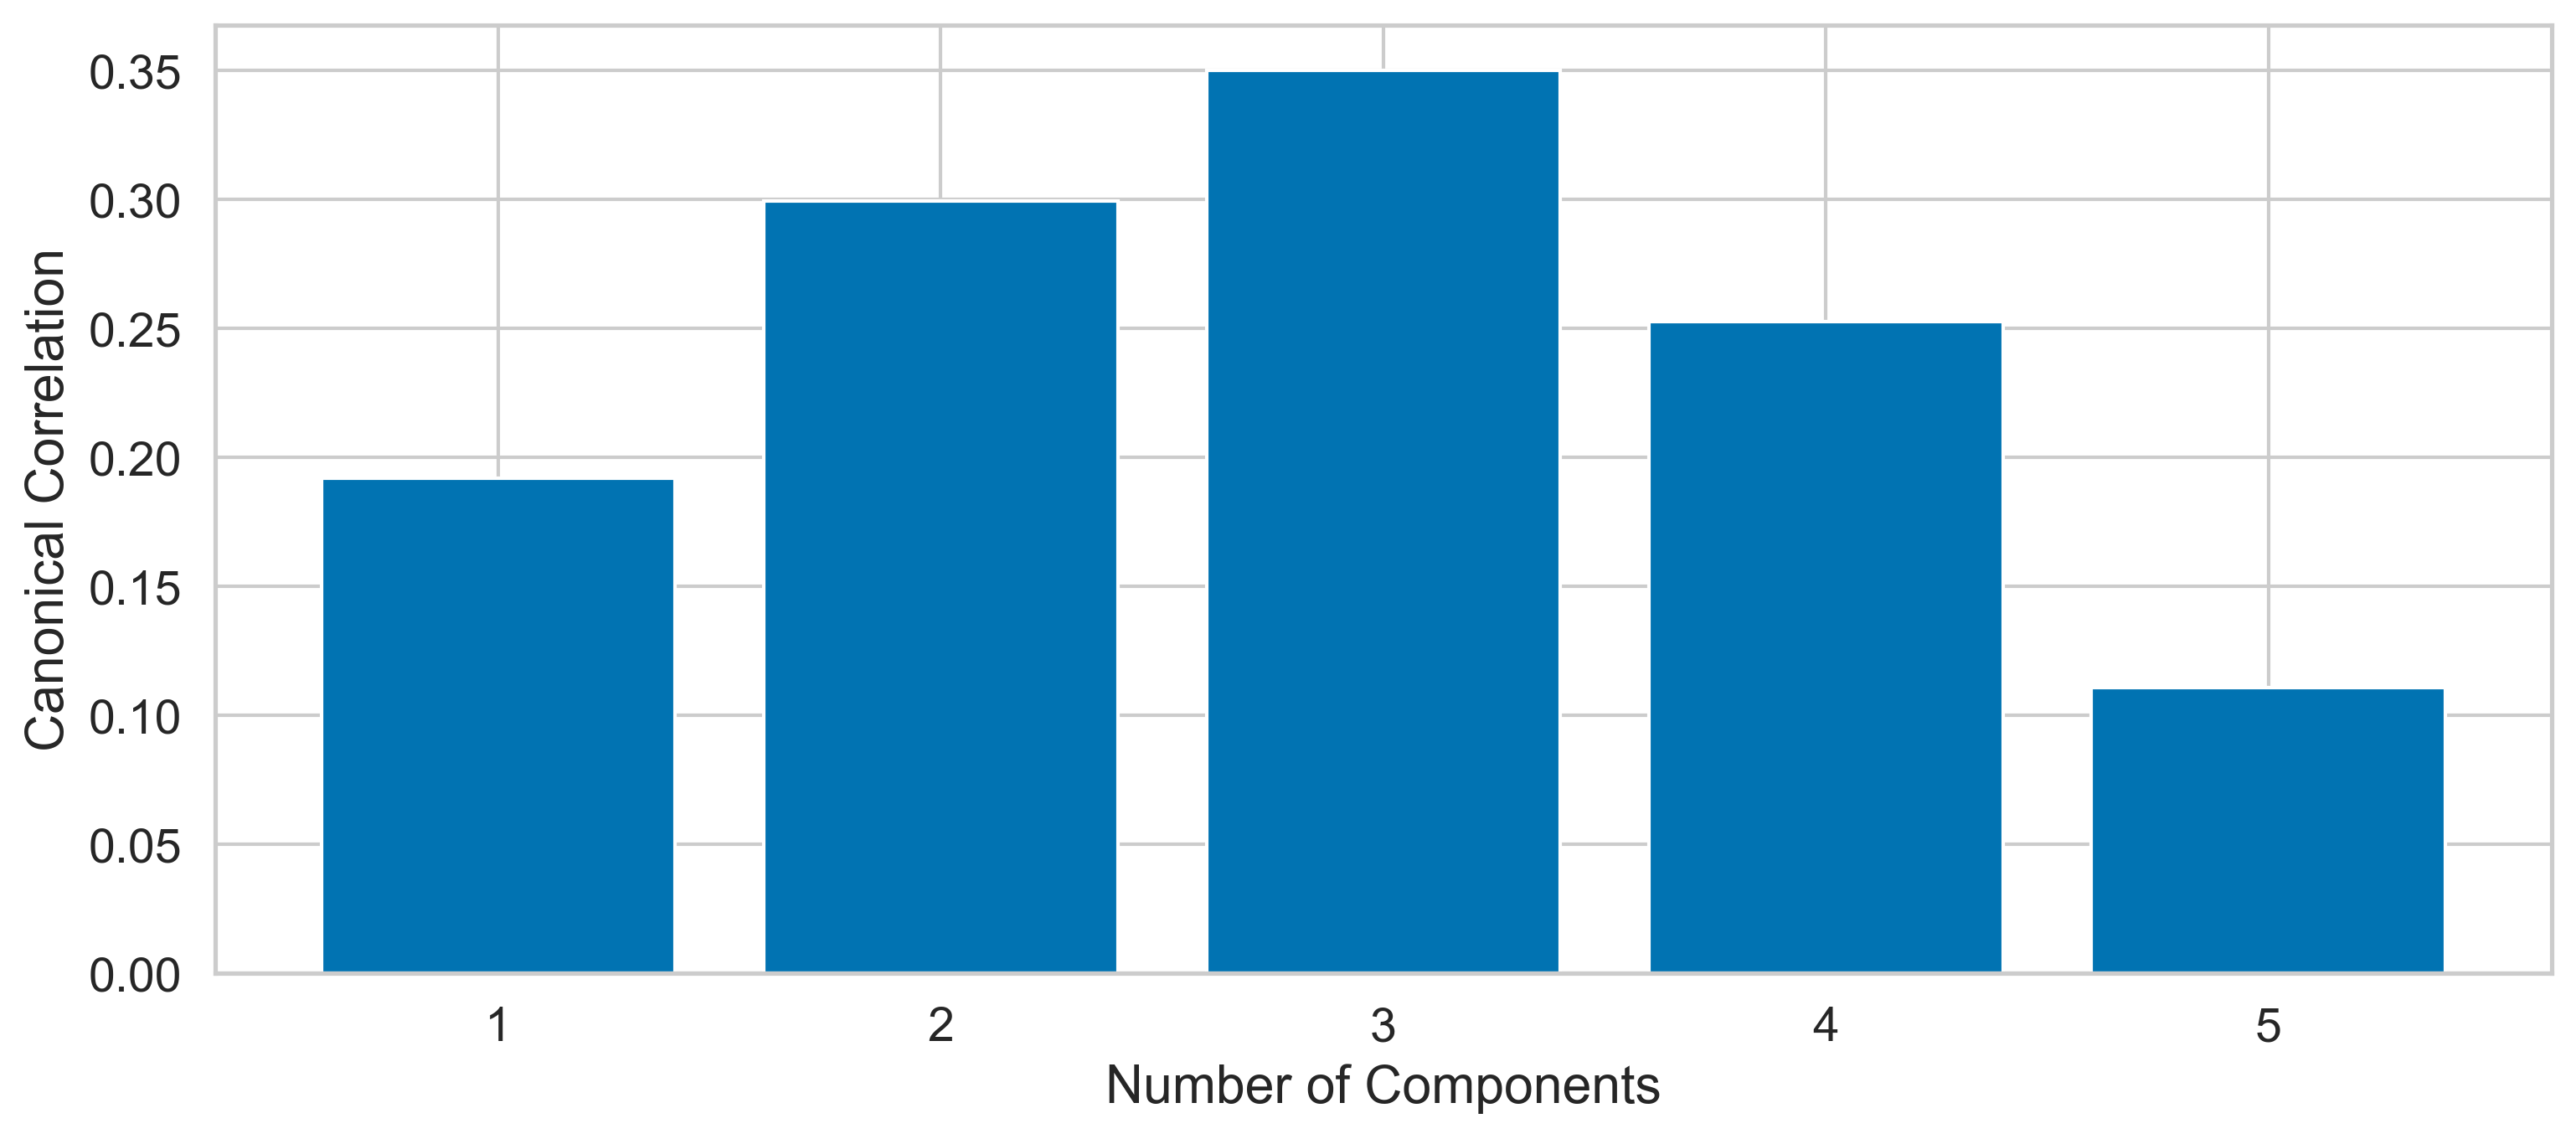
\includegraphics[width=0.8\textwidth]{cca_score.png}
            \end{center}
            \caption{Canonical Correlation between PCA and FF}
            \label{fig:cca_score}
        \end{small}
    \end{figure}

    \item Finally, the PCA loadings are shown in Figure~\ref{fig:pca_loadings}. Again, the market portfolio has decent loadings in all of the 38 industry portfolios. We can see that some principal components capture specific industries. For example, PC8 has higher loadings only on Steam and Water industries, PC2 on Agricultural, Garbage and Government. Factors 3, 4, 9 and 10 look to capture some of the remaining variance left by the market portfolio.

    \begin{figure}[!htbp]
        \begin{small}
            \begin{center}
                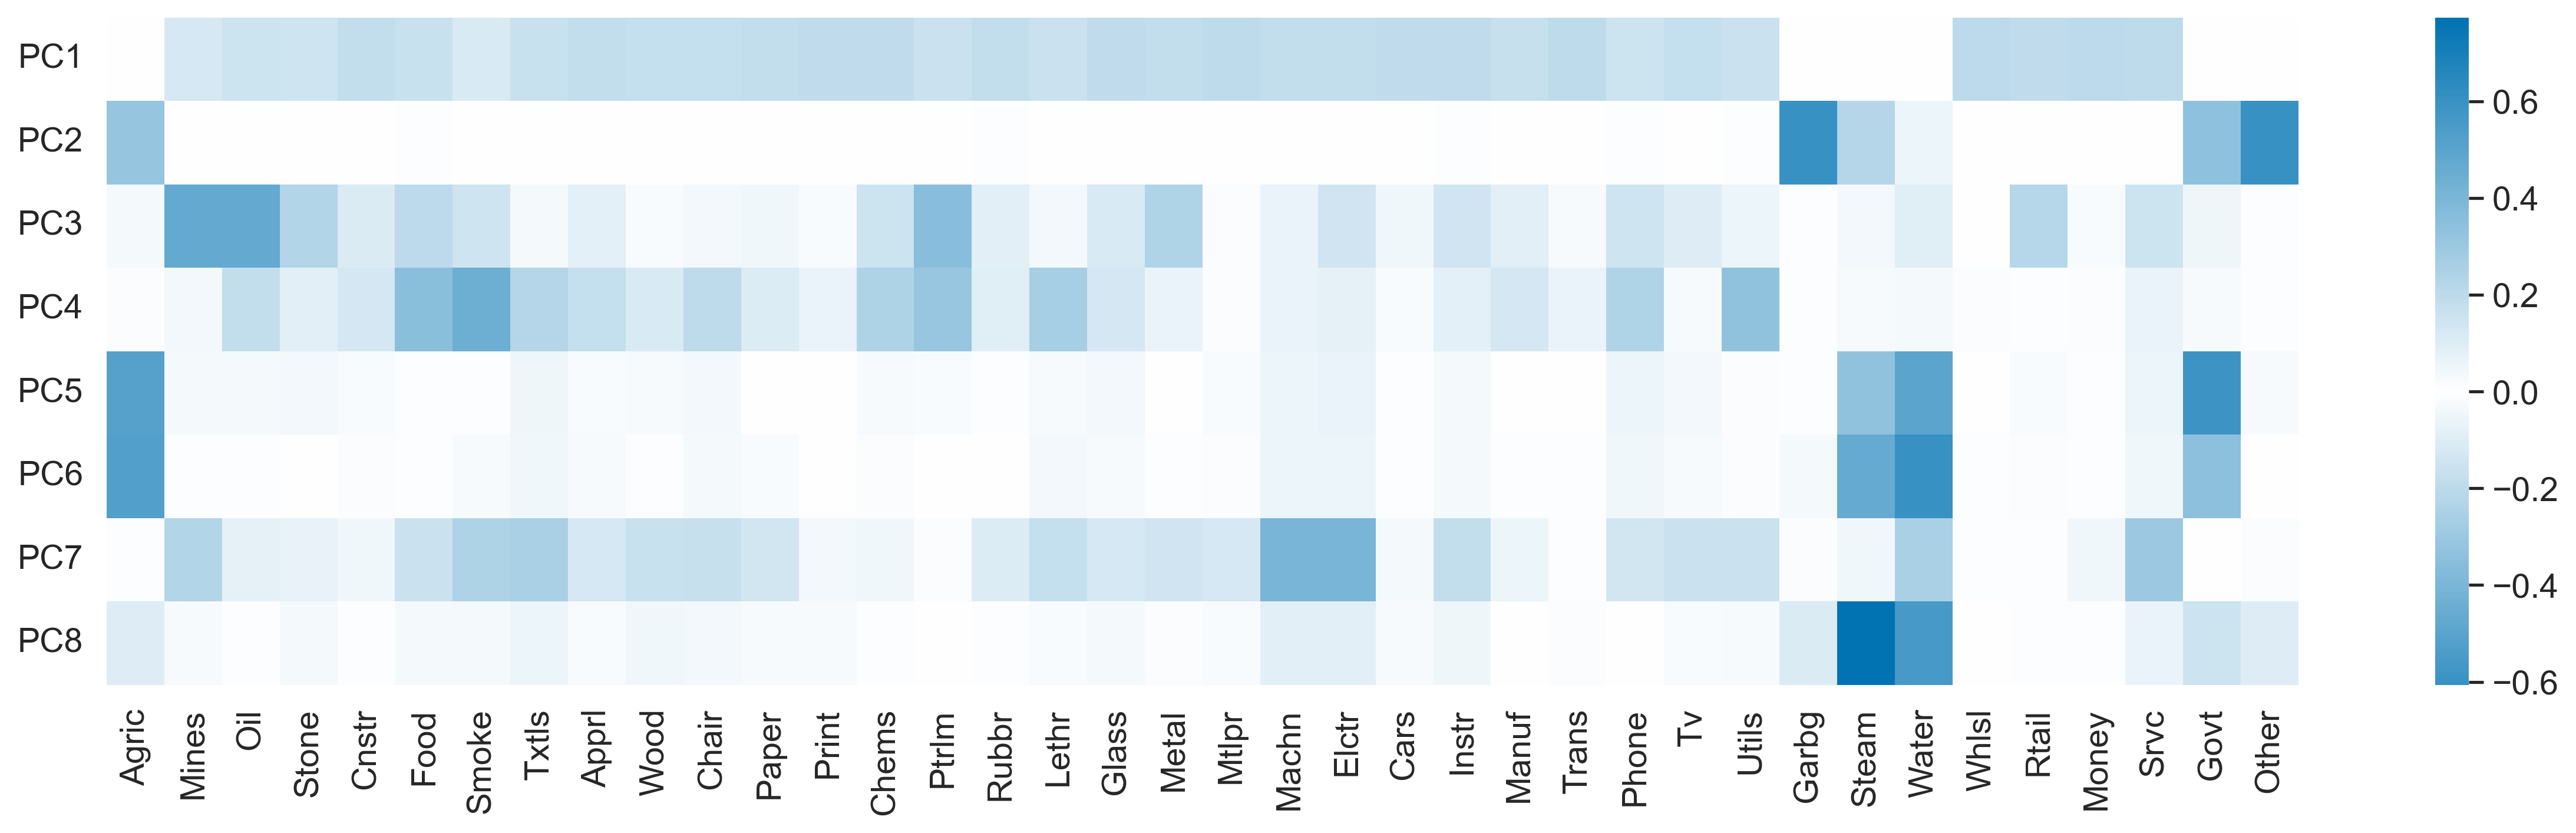
\includegraphics[width=0.95\textwidth]{factor_loadings.png}
            \end{center}
            \caption{Factor Loadings on the PCA}
            \label{fig:pca_loadings}
        \end{small}
    \end{figure}
    
\end{enumerate}
\end{solution}